\chapter{Meteor Detection by Root Mean Square Difference Image Analysis}
\label{chap:image}
\begin{strip}
	\begin{minipage}{\textwidth}
		\begin{abstract}
			I discuss methods of meteor detection by image analysis focusing on root mean square difference, noting structural similarity index, edge detection, and derivatives as alternatives. I provide a quantitative measure of correlation between mean square error image analysis and established methods of radio meteor detection. I find that root mean square difference, as a comparative measure of meteor flux, correlates well with detection counts, suggesting it is a valid method of meteor detection. This provides a basic and easily adaptable alternative to existing software.
		\end{abstract}
	\end{minipage}
\end{strip}
\section{Overview}
The primary method of radio meteor detection is using software to record the signal input, and compare background intensity to signal intensity across the desired frequency. Where there is a large increase in signal intensity, a meteor is considered to have been detected. An alternative to this is image analysis. This method applies a similar technique of recording the signal input, and displaying the result as a `waterfall' plot (figure~\ref{fig:img:waterfall}). Note that the frequency is not the actual frequency, since squelch is applied to the input signal. This output is saved as an image (in a format of the observer's choosing), which can then be analysed to pick out hotspots of colour (depending on the palette used to format the image), distinct edges, or other methods. I discuss these various methods of image analysis.
\begin{figure}
	\centering
	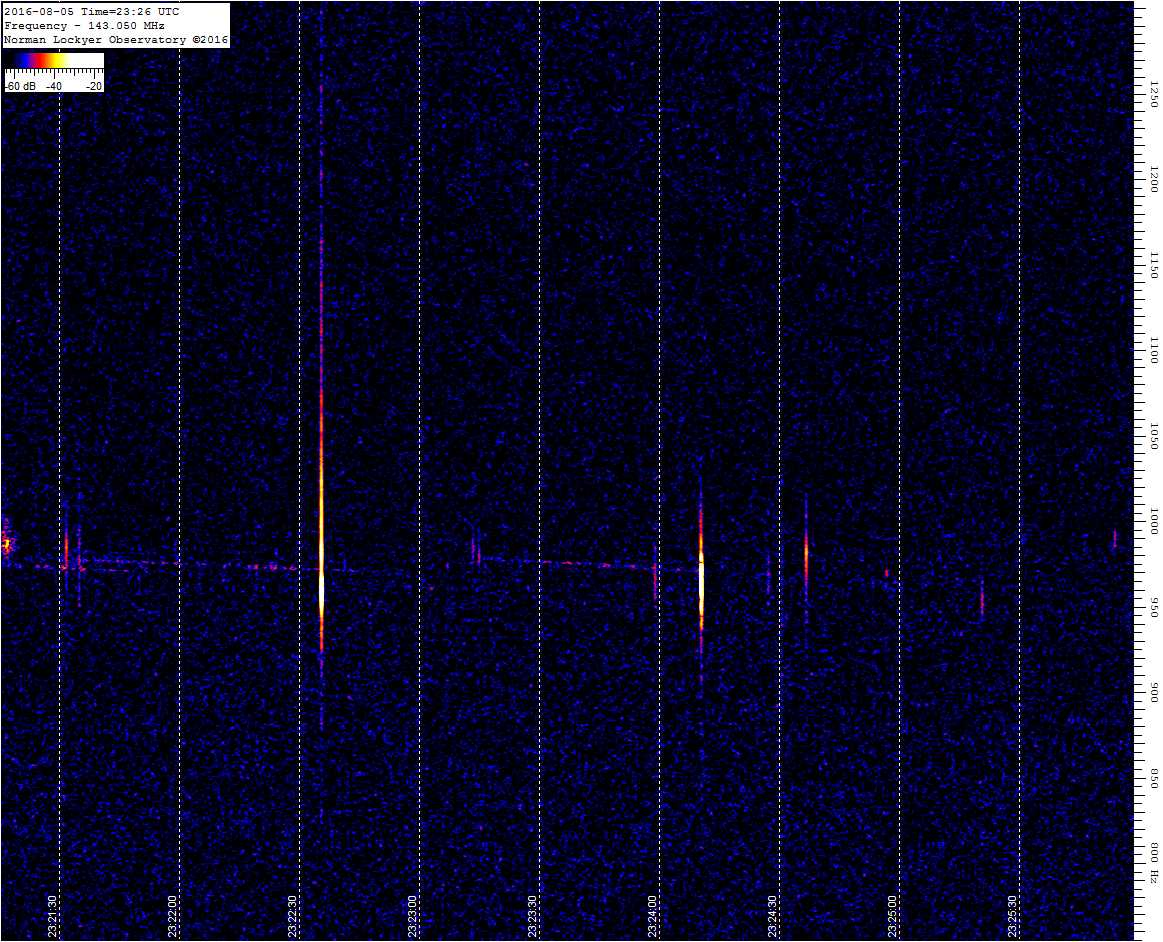
\includegraphics[width=\linewidth]{img/2D}
	\caption{2D waterfall plot from Spectrum Lab v3.0 \cite{speclab}
		\label{fig:img:waterfall}}
\end{figure}
\section{Methodology}
\subsection{Root mean square difference}
The general idea behind my proposed method of root mean square (RMS) difference is to compute the difference between corresponding pixels in two images: the image under consideration, and a reference image. The choice of reference image is somewhat arbitrary, as long as the same reference is used for all computations. The images that will be considered are screenshots automatically taken from SpectrumLab v3.0 \cite{speclab} every minute. The meteor `detection' comes from the change in the RMS difference over time. This change occurs since a meteor is represented as a yellow (or white) streak, which will significantly change the pixel values of the image. The RMS difference is the root mean square of all pixel differences. The value does not indicate exactly how many meteors have been detected, but an increase indicates a greater pixel difference, which itself indicates an increase in signal strength. An increase in signal strength is how radio meteor detection typically takes place, so the results should correlate well.
\paragraph{Repeated images\\}
The input signal moves across the screen, taking 5 minutes to clear the entire window, meaning the same meteor is theoretically `seen' 5 times. However, the RMS difference is a comparative measure rather than exact. The value itself has little meaning, but the change over time should indicate the change in meteor flux. This means that having the same meteor appear multiple times is beneficial, since the value may change by pure chance between each image, but repeated detections of meteors will give a distinct result in the RMS difference.\\
\paragraph{Baseline image generation\\}
The baseline image can be generated in various ways. The aim of generating a baseline should be to minimise differences that do not contribute to the result. Namely, artefacts such as watermarks and scales which cannot be removed automatically. This can be done by averaging as many of the expected comparison images as possible. This will result in an image similar to figure~\ref{fig:img:avg}. A better baseline will be produced by including more images: I have used a sample of an entire day (1440 images) to produce figure~\ref{fig:img:avg}. Alternative baseline images are as simple as a completely black image. As long as the same baseline is used, the choice is arbitrary.
\begin{figure}
	\centering
	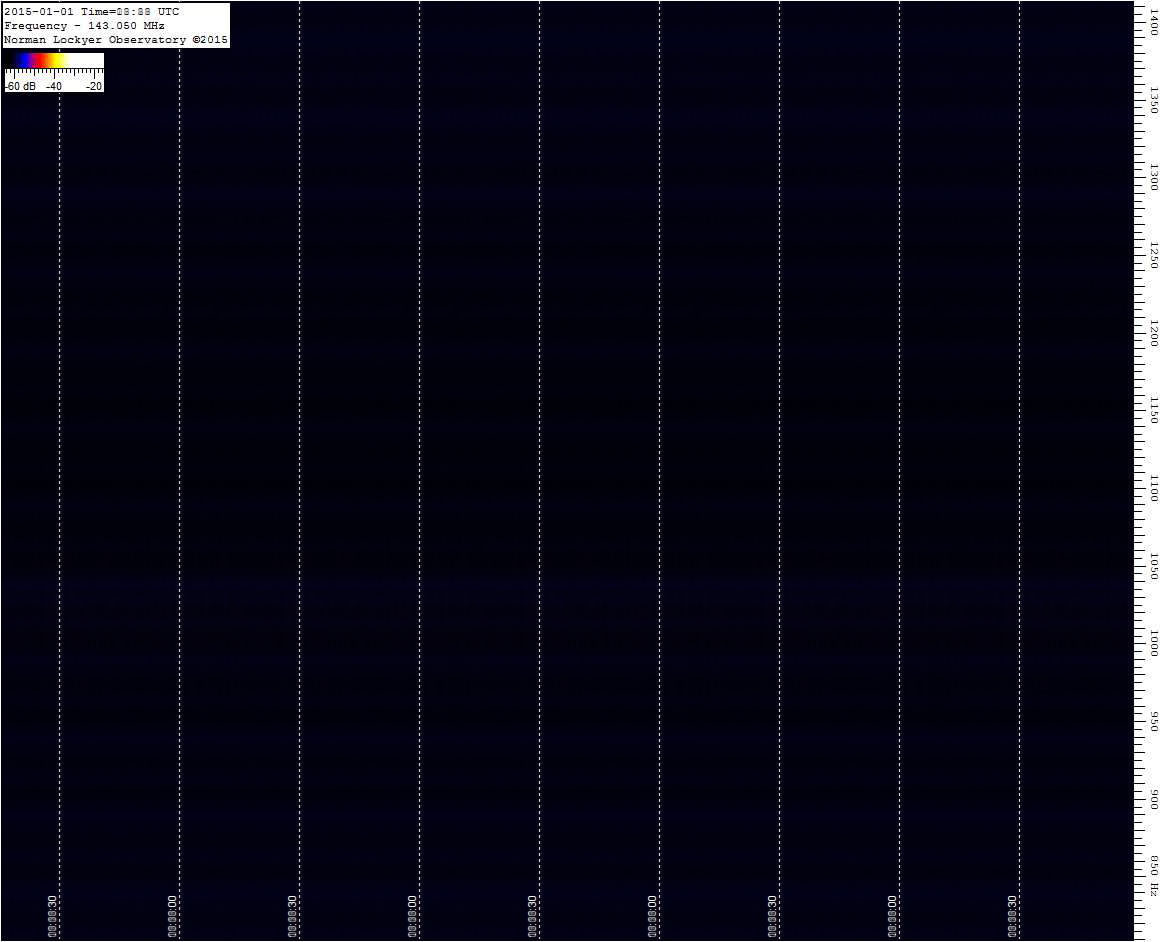
\includegraphics[width=\linewidth]{img/average}
	\caption{Average image for comparison baseline
		\label{fig:img:avg}}
\end{figure}
\paragraph{RMS calculation\\}
For my own method, the calculation is made using Python. Before the RMS difference can be calculated, a histogram of the image must be generated. This contains all possible values of the pixel values, and their associated differences between the considered image and baseline image. The root mean square of this histogram is then taken, which gives the desired result. This is repeated for each image and stored in a place of the observer's choosing (a text file makes the most sense). 
\paragraph{RMOB comparison\\}
In order to test the effectiveness of this new method, I will compare the results with hourly detection counts collected using RMOB \cite{rmob}, for the same location, where the program running the RMS difference is implemented: the Norman Lockyer Observatory, in Devon. The RMS values are present for every minute, whereas RMOB counts are for an entire hour. In order to solve this, all the RMS differences for an hour are averaged.
\section{Results}
\subsection{Data}
The RMOB hourly detection counts are shown in figure~\ref{fig:img:rmob}. All available RMS values are shown in figure~\ref{fig:img:rms}. There is a large gap in detection count data, which reduces the size of the data set which can be compared, however there are still 2833 pairs of values. The range of this comparison is from 2014-11-01 to 2016-11-17. 

\begin{figure}[h!]
	\centering
	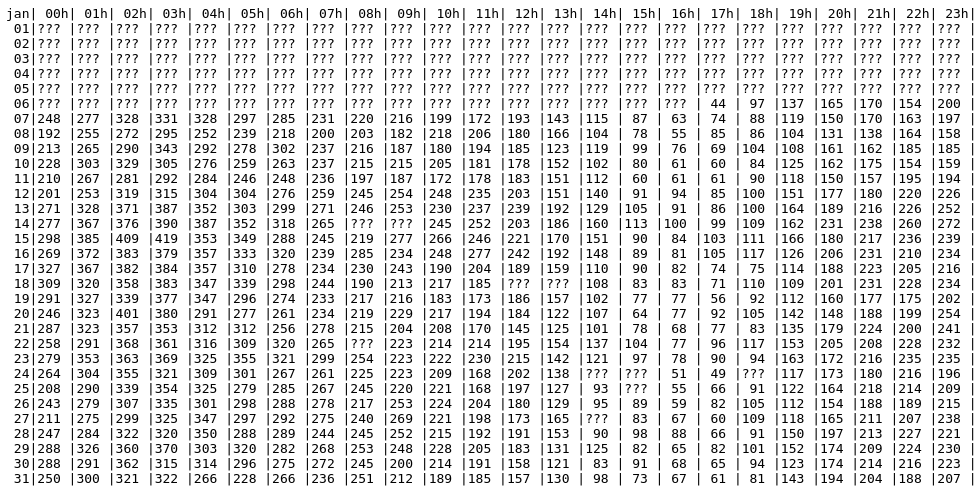
\includegraphics[width=\linewidth]{img/rmob}
	\caption{Meteor detection count (RMOB count) for NLO, Devon
		\label{fig:img:rmob}}
\end{figure}
It is clear from figure~\ref{fig:img:rms} that there are erroneous results for RMS differences. These can occur when the antenna is moved by wind (or by observer error) which dramatically increases the noise in the waterfall plot. This noise manifests itself as an increased blue background since there are more `spikes' for frequencies outside the receiving frequency. Until the antenna is moved back to the correct position, the increased noise will persist and results in a clear offset that can be seen in figure~\ref{fig:img:rms}. Other situations, such as a faulty cable or incorrect software settings, can cause similar problems.
\begin{figure}[h!]
	\centering
	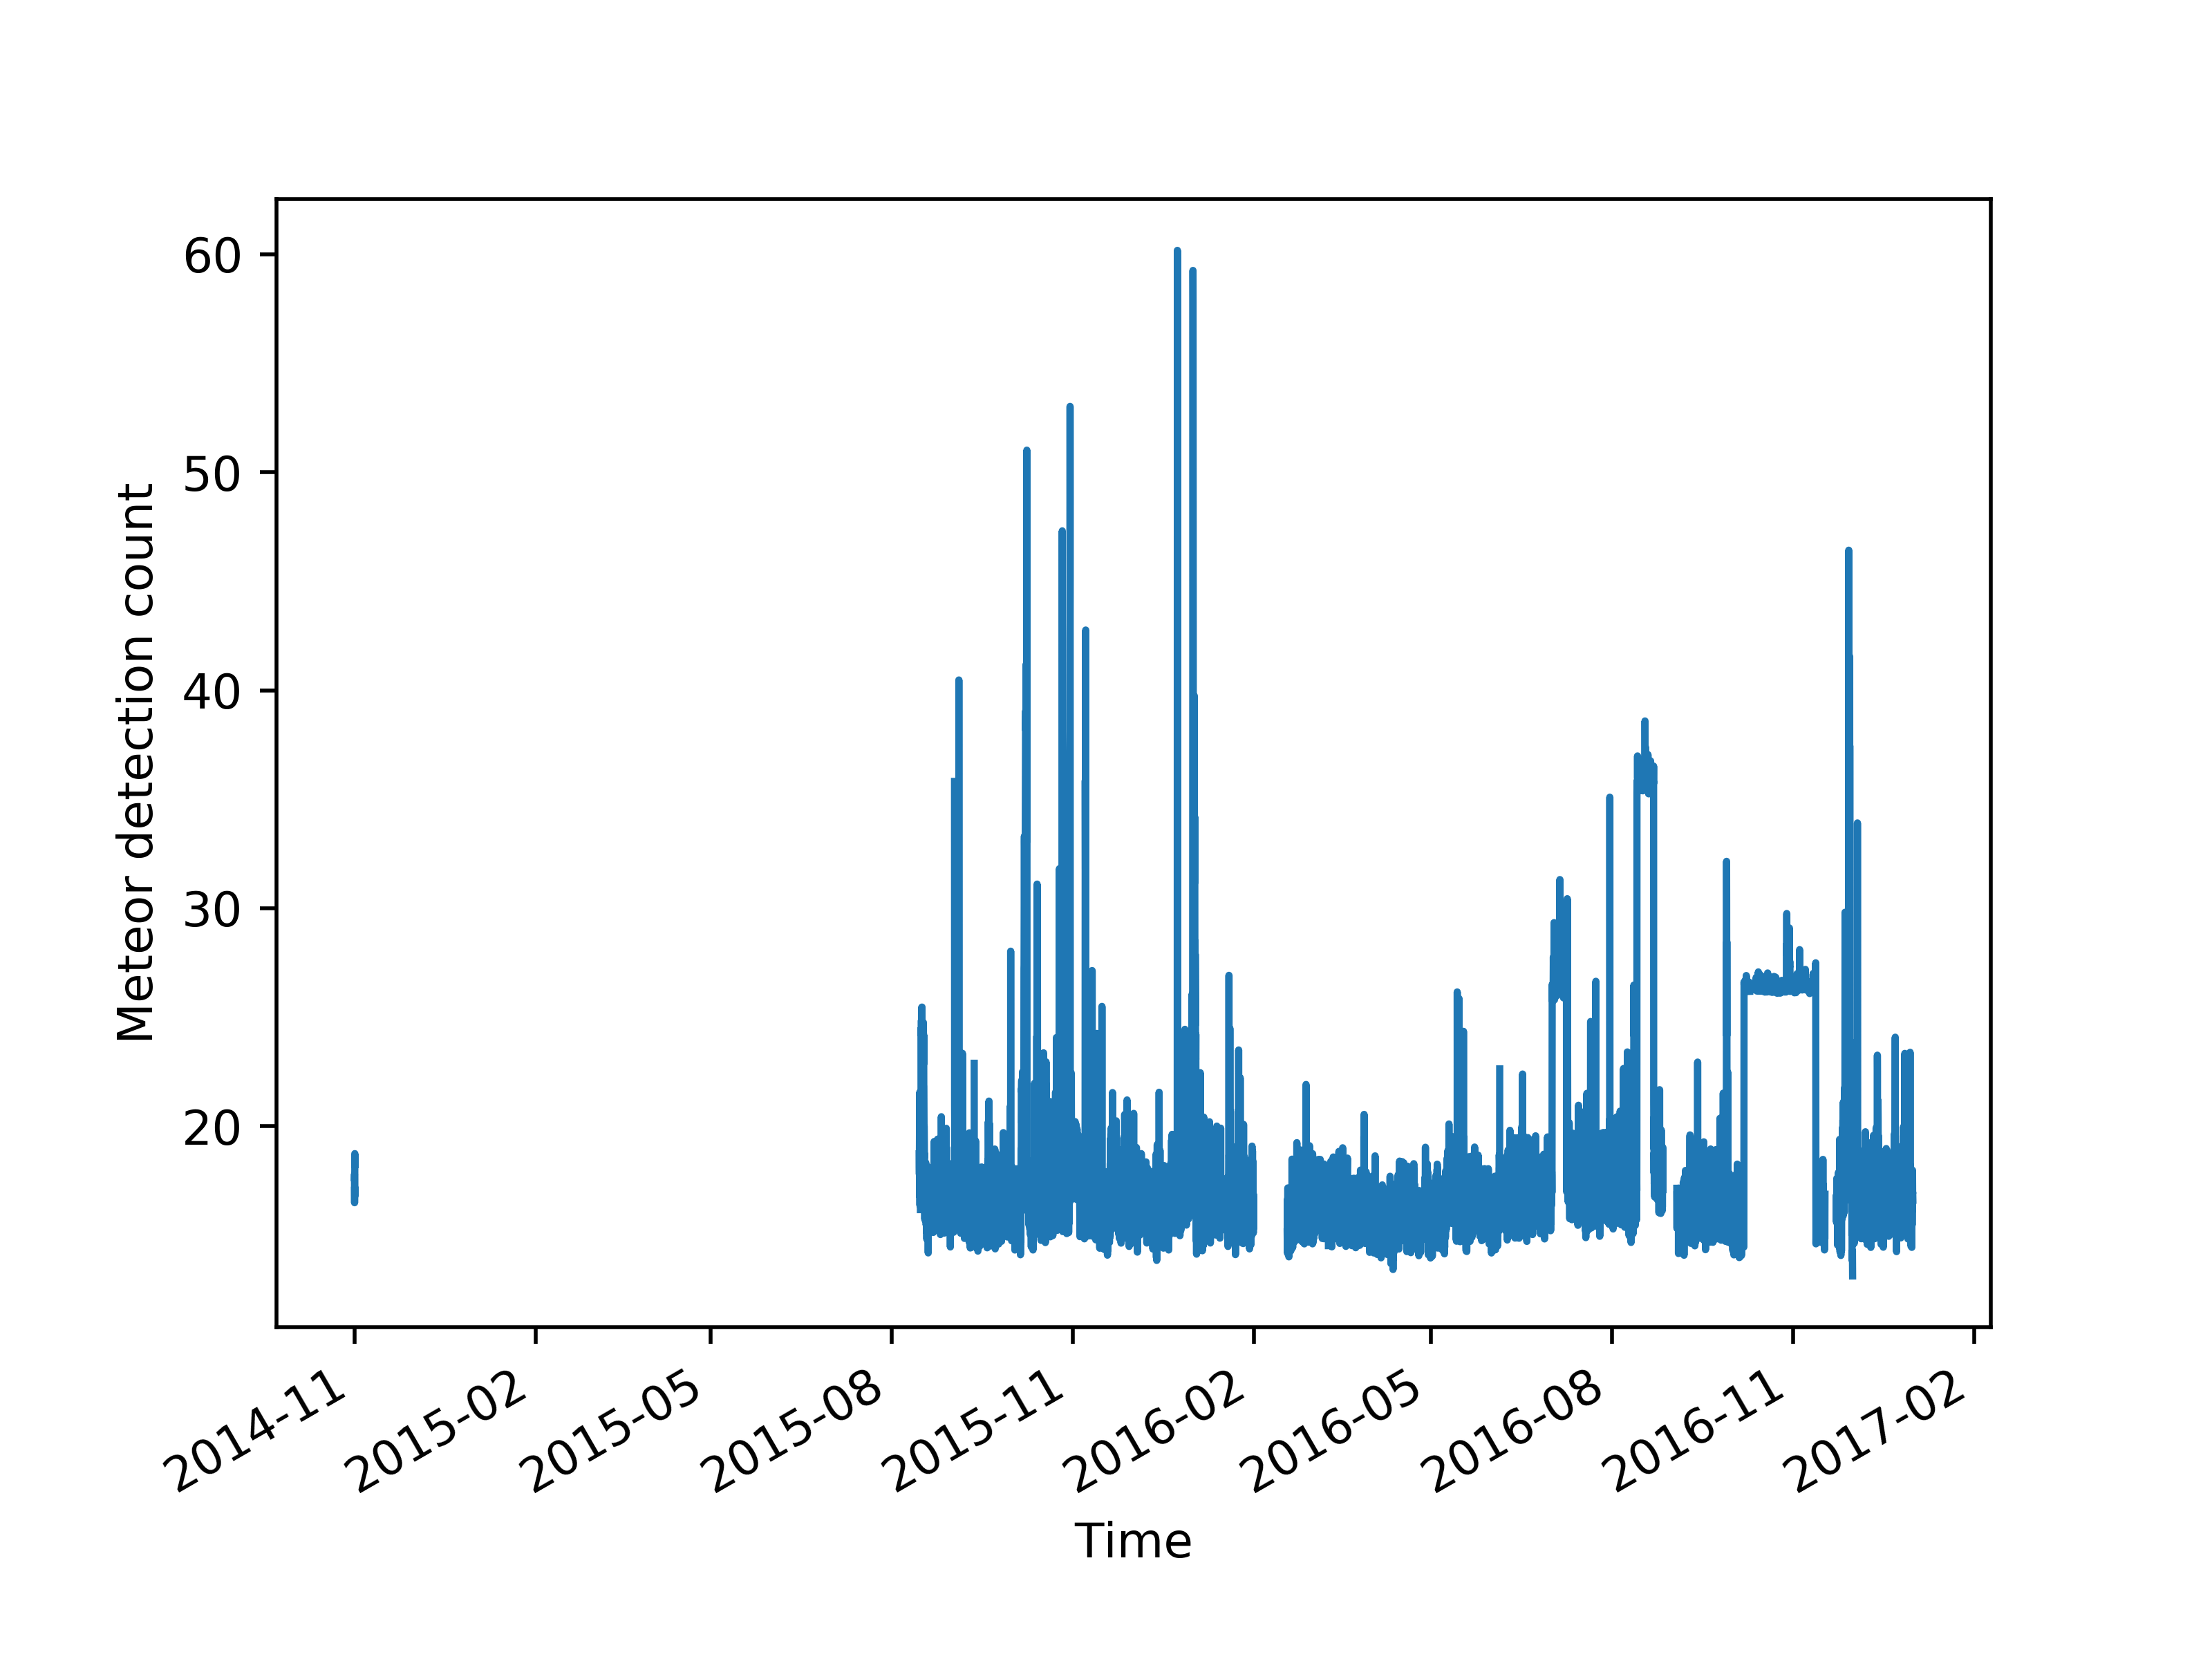
\includegraphics[width=\linewidth]{img/mse}
	\caption{Root mean square difference against baseline for NLO, Devon
		\label{fig:img:rms}}
\end{figure}

\subsection{Correlation}
Figure~\ref{fig:img:before} shows a scatter graph of the RMS difference against the RMOB counts. The periods with erroneous data can clearly be seen, as well as a correlation between the two sets. Even within the erroneous periods, a correlation is seen, though to a lesser extent. This supports the idea that there is only an offset, and can likely be accounted for. However, in order to achieve a true reflection of the correlation between the two sets, I removed the erroneous data, resulting in figure~\ref{fig:img:after}.
\begin{figure}[h!]
	\centering
	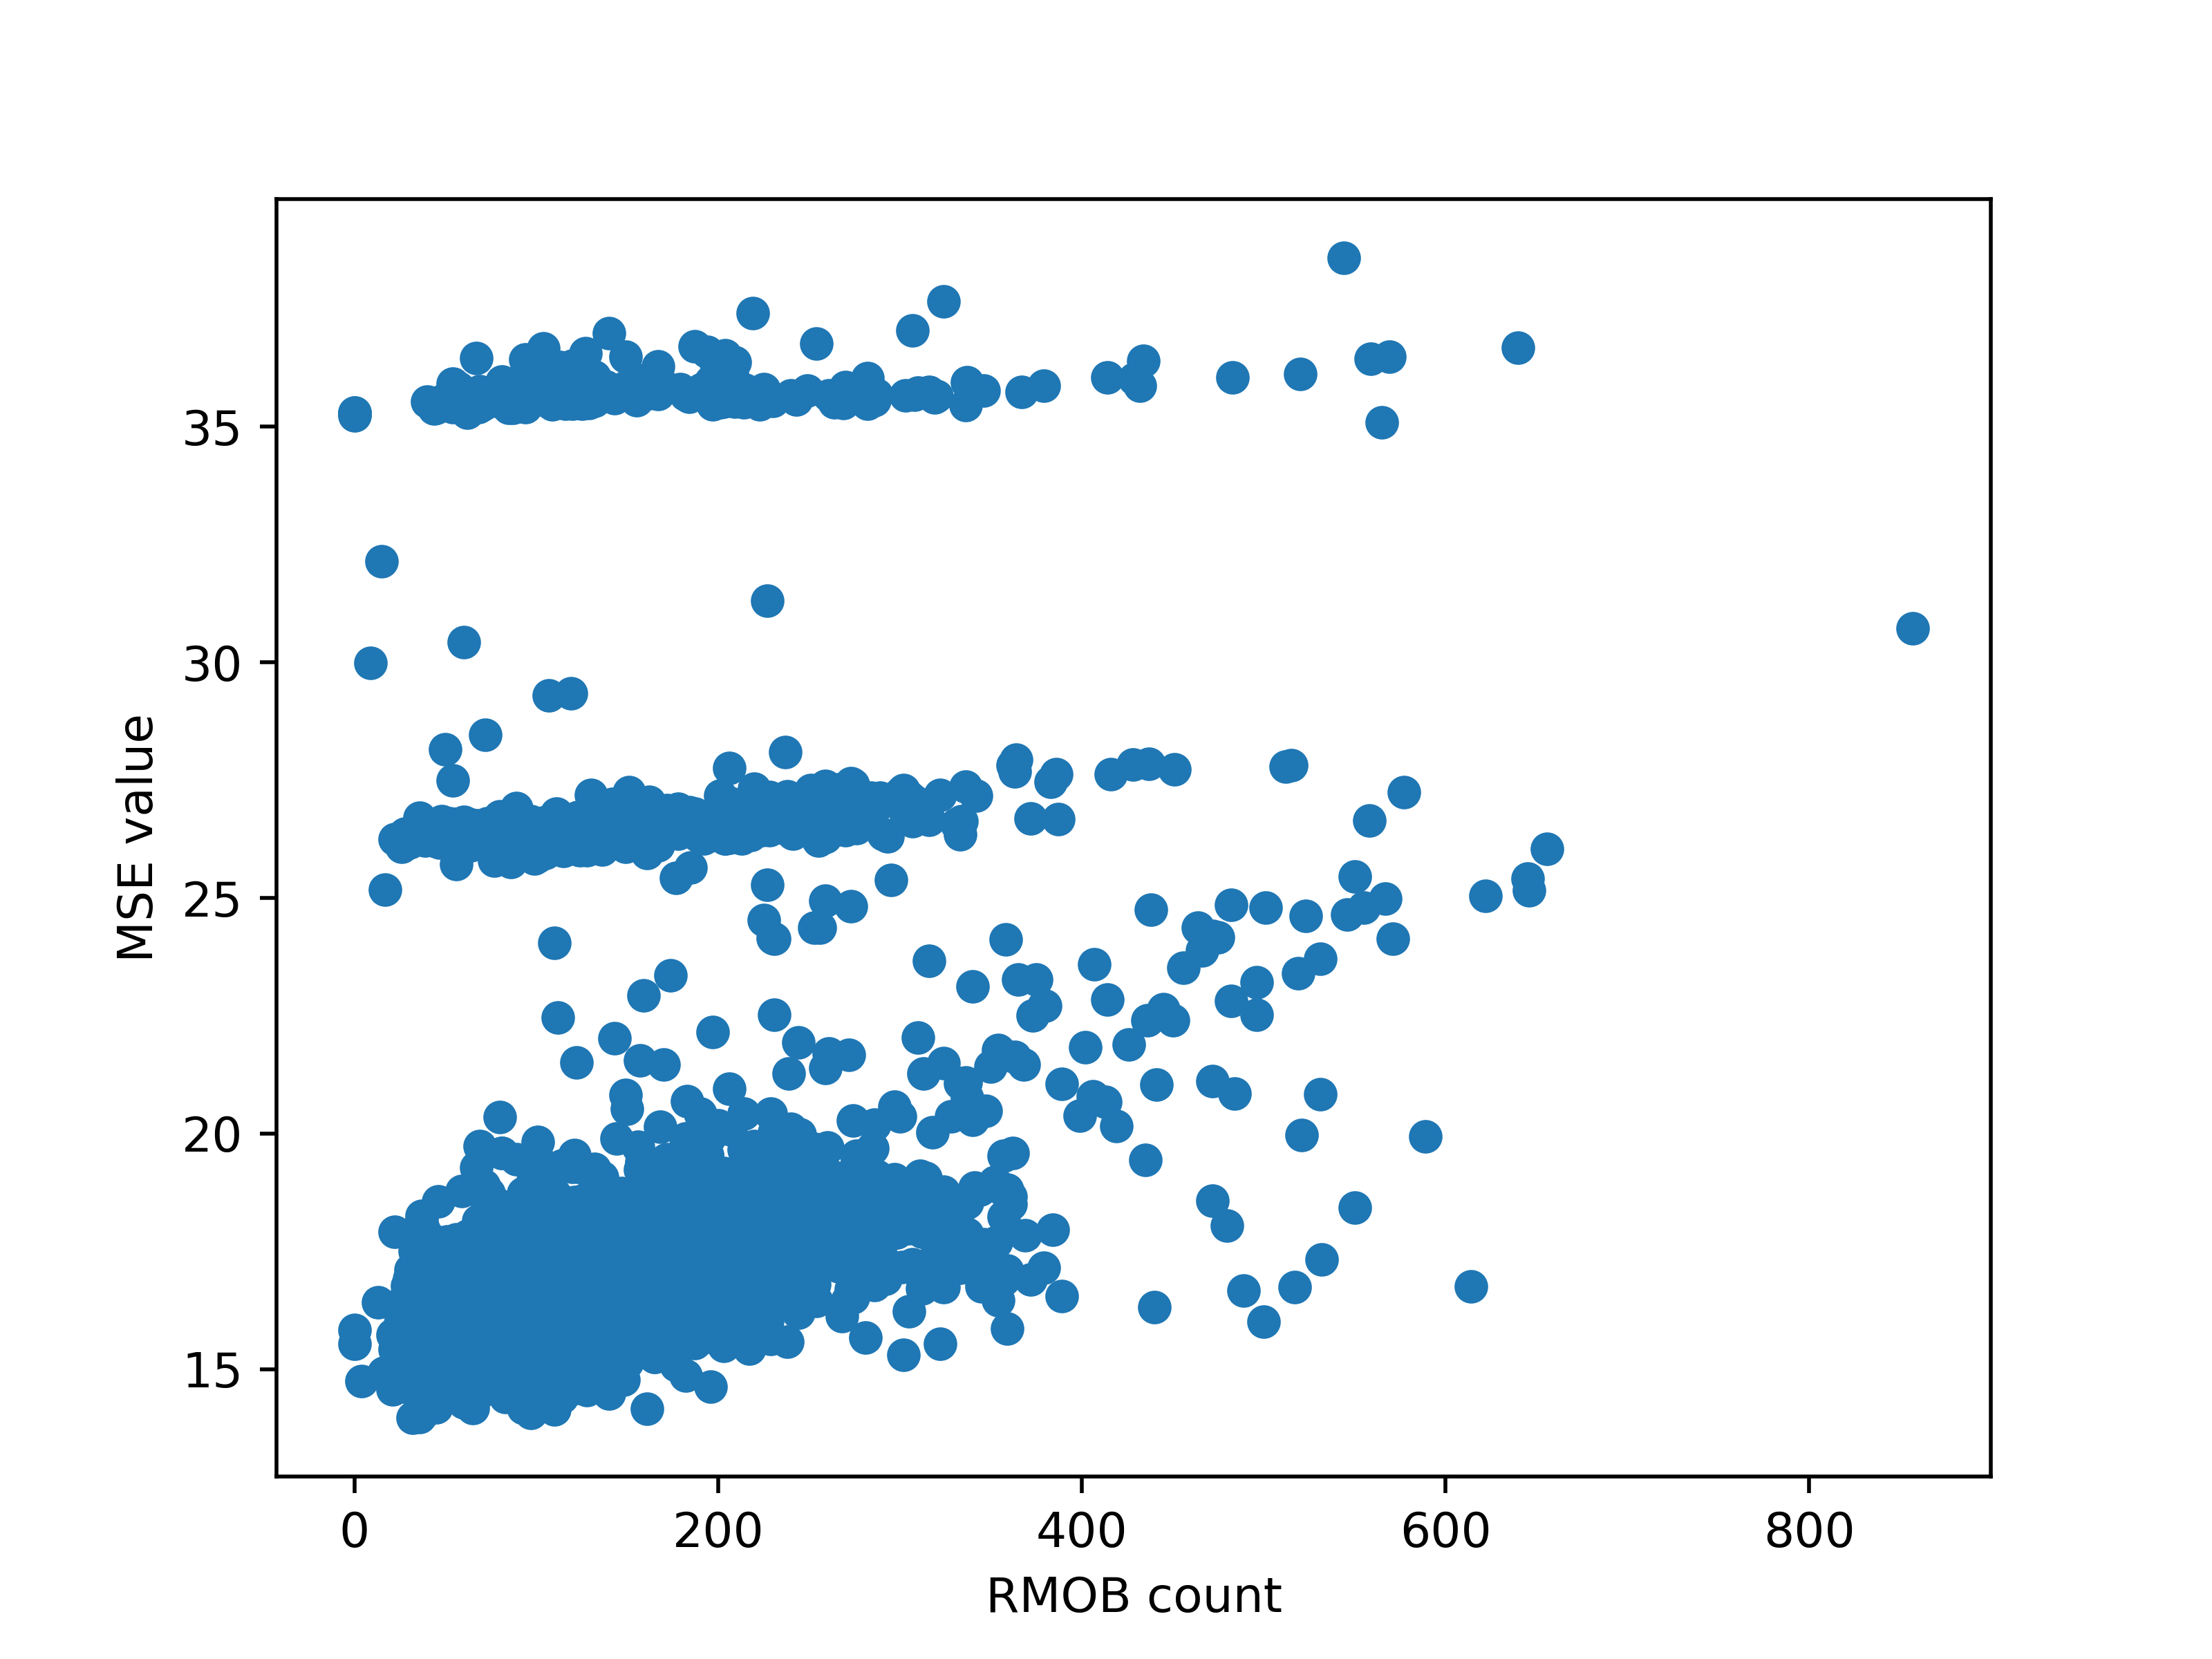
\includegraphics[width=\linewidth]{img/before}
	\caption{RMOB counts against RMS difference, including erroneous periods
		\label{fig:img:before}}
\end{figure}
In the absence of the erroneous data, the correlation becomes clearer. There are, of course, some values that do not appear to be well correlated but there is an apparent overall trend. There are 2042 pairs remaining in the data set. Using Pearson Moment Correlation Coefficient (PMCC), $r = 0.6165$, with a p-value of $4.05 \times 10^{-214}$. Therefore, with a 1\% level of significance, there is evidence to suggest there is a correlation between the two sets. The value of $r$ indicates that there is a strong positive correlation.
\begin{figure}[h!]
	\centering
	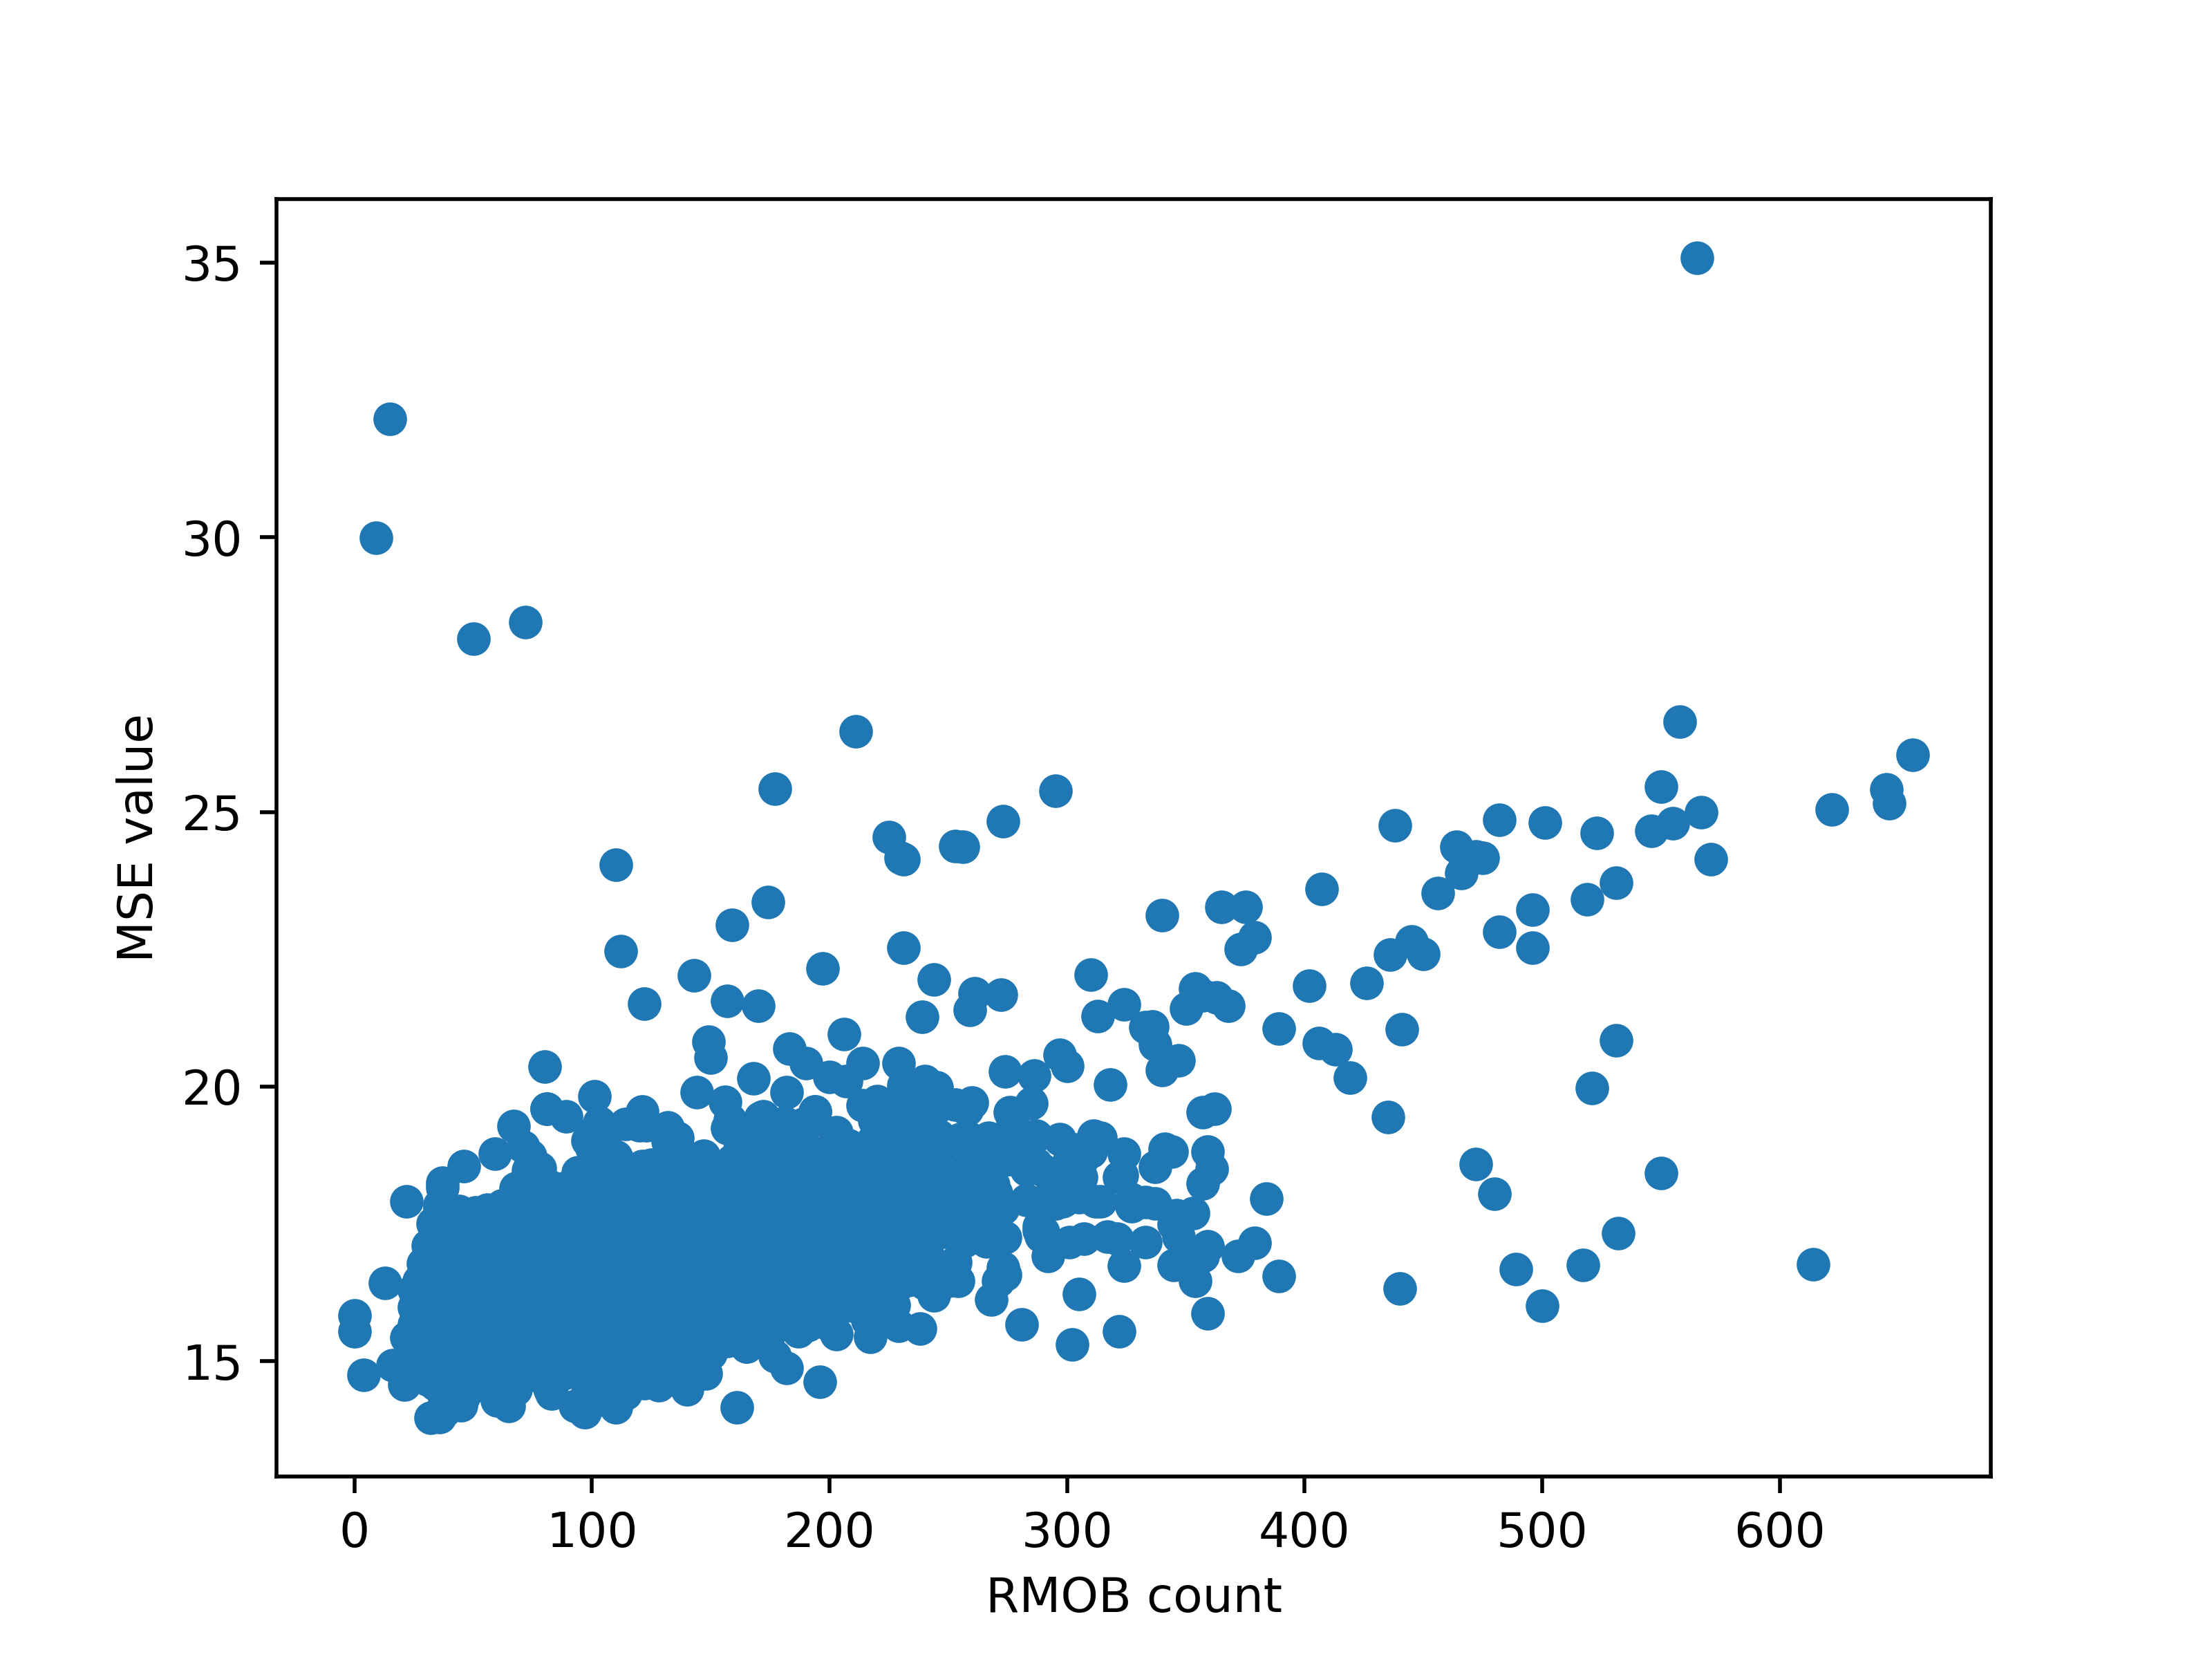
\includegraphics[width=\linewidth]{img/after}
	\caption{RMOB counts against RMS difference, excluding erroneous periods
		\label{fig:img:after}}
\end{figure}

\section{Discussion}
\subsection{RMS difference}
It is clear from the results that there is positive correlation, suggesting that the method is valid as a comparative measure of meteor flux. However, there are improvements that can be made to the method.
\paragraph{Image format\\}
The images that are analysed in this study, are saved with a JPEG format at 50\% quality. Saving as a bitmap would be much more effective, since compression would not create artefacts nor remove data that is important. This does, however, raise issues of memory space, since saving 1440 bitmap images a day will quickly fill up most storage. The best option is to process the images as bitmap, then save as JPEG.
\paragraph{Removing watermarks\\}
Although an average image baseline was used to remove the influence of watermarks, simply removing them is best. This can either be done using the software that creates the images, or an image processing technique. Removal of these watermarks \& scales, variables can be further isolated, meaning the only data that should change between images is the signal being studied, improving the accuracy of results.
\paragraph{Frequency isolation\\}
Theoretically, the only part of the image that should be compared is the main frequency $\pm$ the width of the sideband (depending on whether upper or lower sideband is used). This would negate some influence of increased noise, meaning erroneous periods that occurred in the data I used are not an issue. In fact, the area of the image could be decreased further still, since the furthest edges of the sideband do not contribute much to the overall RMS difference, since the peak intensity is towards the carrier wave frequency.
\paragraph{Relative measure\\}
An alternative method of negating the influence of noise is a relative measure of the RMS difference. By considering the most recent RMS differences, or by making a post-analysis pass and comparing against values before {\it and} after each value, the RMS difference can be normalised so that any offsets are removed.
\paragraph{Meteor count interpolation\\}
Since there appears to be a correlation in the data, using a regression line would allow interpolation of meteor counts based on the RMS difference. Of course, this will have some inherent error, but as an estimation it may be useful.
\subsection{Alternative methods}
\paragraph{Structural similarity index measure\\}
Structural similarity (SSIM) \cite{ssim} is designed to be a better alternative to RMS difference. It is a `full reference' method, meaning it requires a reference image, much like RMS difference. It measures {\it perceived} change in the structure of the image. This is applicable to detecting meteors from images since the changes between an image with and without a meteor are significant in terms of structure. A meteor, in a waterfall plot, is seen as a large yellow streak. This will be easily picked up by the SSIM method since it includes a measure of variance, which will change if large pixel values are present in the image compared to a baseline. SSIM would provide a comparative measure much like RMS difference: the number of meteors in the image is not calculated, only a comparative measure of meteor flux.
\paragraph{Edge \& blob detection\\}
Edge detection is the process of identifying edges in an image. In combination with blob detection, the outlines of `blobs' can be picked out from an image. For meteor detection this is advantageous: since meteors are represented as distinct coloured streaks, a blob with a certain shape is likely to be a meteor. This shape can be analysed using a convolution. Areas that are picked up best by the convolution, blob and edge detection can be considered as meteors. Counting the numbers of meteors will give results that can much more easily be compared to RMOB counts, indicating the effectiveness of the method.
\paragraph{Derivative method\\}
Finally, I propose using derivative methods to pick out maxima in an image. This can be done by considering each row of pixels in the image, as well as each column, and calculating derivatives (most likely by forward difference), so that maxima can be identified. Picking out maxima that occur in both directions indicates a significant peak in the image. Through analysis of these results, a threshold can be picked out for the gradient required for a maximum to be considered a meteor.
\section{Conclusion}
Methods of meteor detection by image analysis, using root mean square difference, correlate well with hourly detection counts at a 1\% significance level. This provides an alternative method to standard techniques of radio meteor detection, which can easily be implemented and modified to an observer's use. I have discussed ways to improve this method to give more accurate results, providing a more valid comparative measure of meteor flux. As well as this, I have discussed alternative methods of image analysis that can provide hourly counts, as well as methods that could provide better comparative measures than RMS difference.